%************************************************
\chapter{Discussion}\label{p04:discussion}
%************************************************
After the implementation of session tracking, useful information about time and quality of work can be presented to teachers and students. Example of questions and analysis that can now be performed with the session tracking are presented in this chapter.
With this knowledge they can adjust their teaching strategy and have a better understanding of how the class is using the system.

\section{Reading session}

By visualizing the amount of time spent for the students in a class, we can detect "islands" of activity common for the whole class (Figure \ref{fig:class_heatmap_by_date}). These can be explained with a visualization by week day. In Figure \ref{fig:class_heatmap_by_weekday} we can confirm that the students are mostly actively reading on Sundays and Mondays.

\begin{figure}[bth]
	\myfloatalign
	\subfloat[Heat map of time spent by day and user in a class]
	{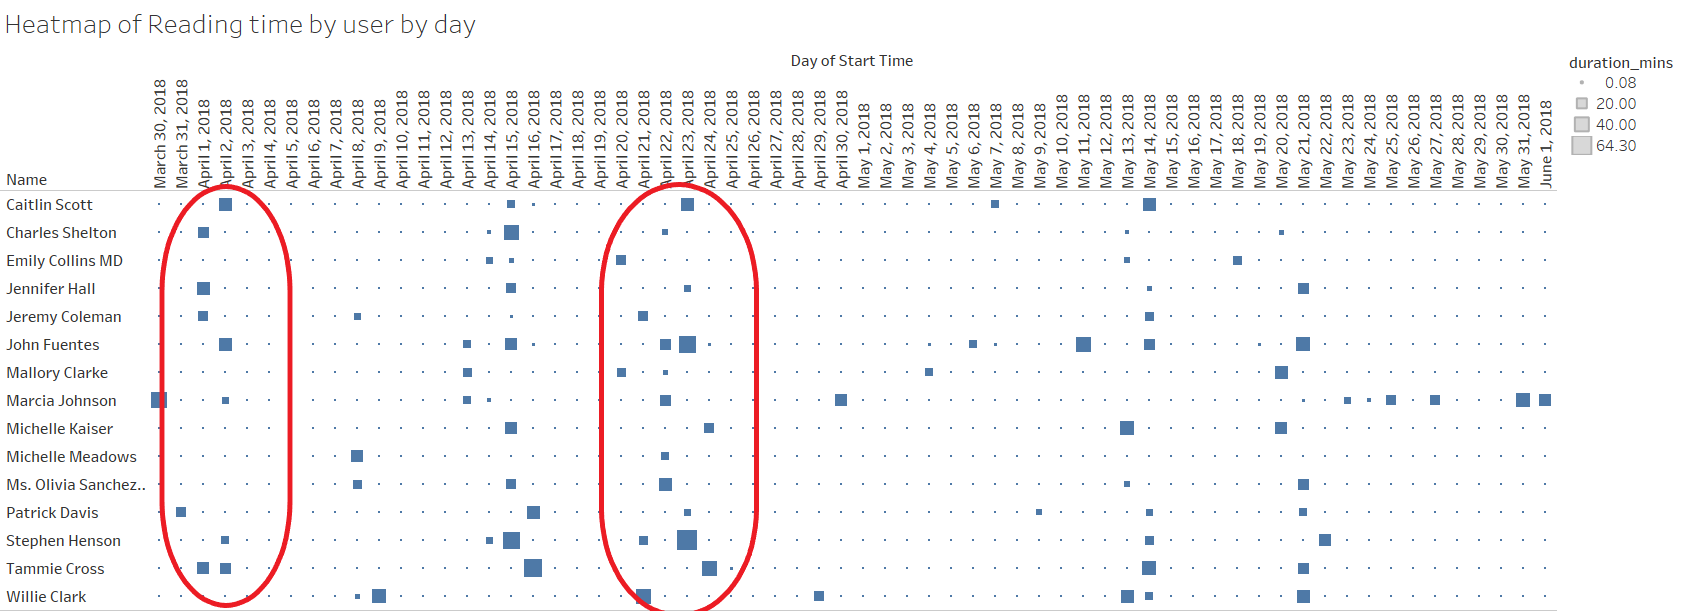
\includegraphics[width=.45\linewidth]{gfx/Heatmap_by_user}\label{fig:class_heatmap_by_date}} \quad 
	\subfloat[Heat map of time spent by weekday and user in a class]
	{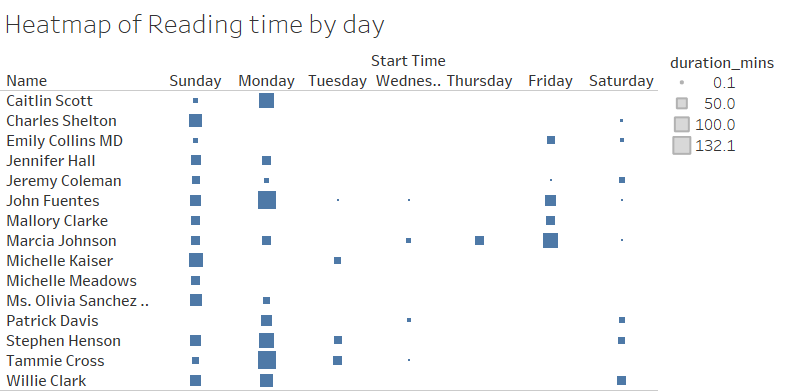
\includegraphics[width=.45\linewidth]{gfx/Reading_time_by_weekday}\label{fig:class_heatmap_by_weekday}} \quad
	\caption{Total time spent by a class, analyzed by date}
\end{figure}


Since the reading sessions are associated to an article, an analysis of the time spent by article can be performed. In Figure \ref{fig:treemap_by_article} we display the total amount of time spent by a class of students learning Dutch. With this information the teacher can observe which articles are the ones that most students have read, and also from which source they read, so a further discussion in class about the content can be done.

\begin{figure}[h]
	\centering
	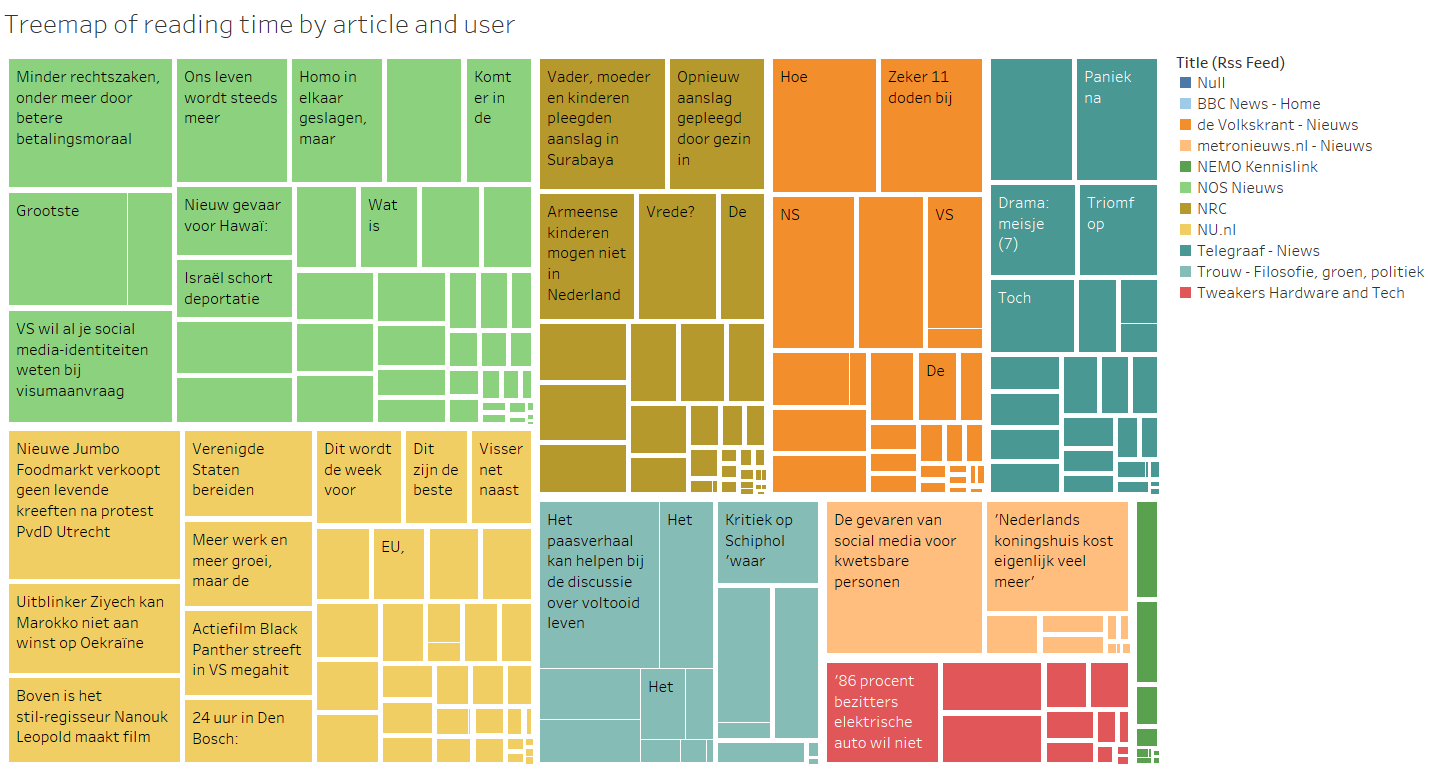
\includegraphics[width=1\linewidth]{gfx/Treemap_by_article}
	\caption{Treemap of time spent by article. The color indicates the source of the article. Each block represents a user and the size represents the total time spent by a user on that article}
	\label{fig:treemap_by_article}
\end{figure}

%An alternative way of grasping an idea about text difficulty and quality of work can be done based on the time students spend on average reading an article. In Figure \ref{fig:boxplot_by_article}, we can observe that most of the articles were read during less than ten minutes, amongst which the majority are concentrated in less than 4 minutes sessions.
%
%\begin{figure}[h]
%	\centering
%	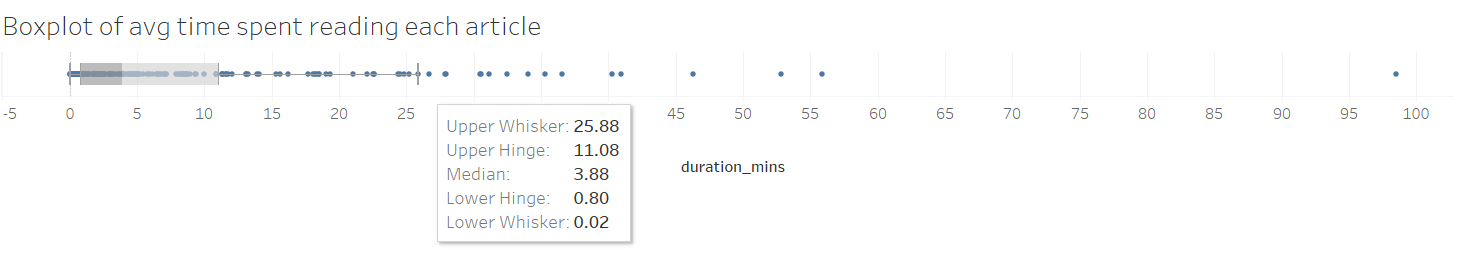
\includegraphics[width=0.7\linewidth]{gfx/avg_time_spent_by_article}
%	\caption{Box plot of the average time required to read an article. It shows that most articles are read in less than 10 minutes and that there are some articles that take more time}
%	\label{fig:boxplot_by_article}
%\end{figure}

And at the individual level, the user can visualize and understand his own work, in order to be aware of his own progress. In Figure \ref{fig:Personal_dashboard}, an example of a dashboard containing the information that could be relevant for a user is displayed.

\begin{figure}[!htb]
	\centering
	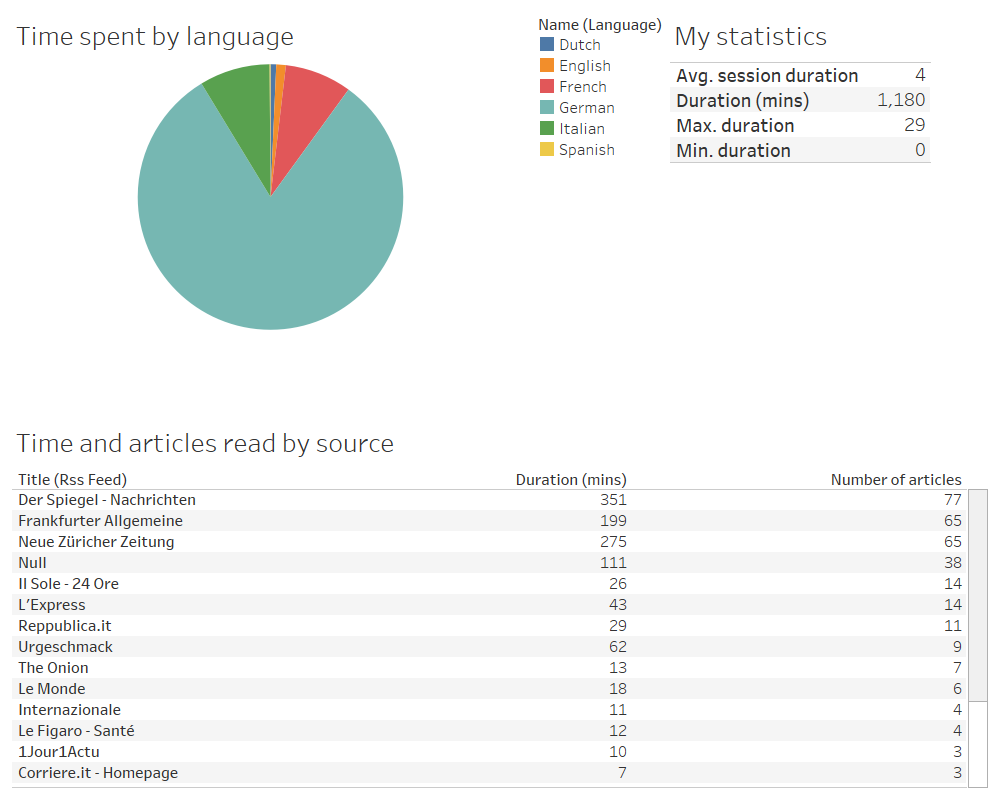
\includegraphics[width=1\linewidth]{gfx/Personal_dashboard}
	\caption{Dashboard displaying individual statistics about reading habbits}
	\label{fig:Personal_dashboard}
\end{figure}



\section{Exercise session}
Typical questions related to the exercises are how much time has the student been practicing? Do they practice daily? For how long? Etc. In this chapter a list of analysis based on time spent on exercises is shown and discussed.

The first question is how much time the class is spending on practicing their vocabulary? With a simple bar chart we can visualize and compare how much time in total has the class spent practicing, and also who has been putting more effort on it. As we can observe in Figure \ref{fig:Total_exercise_time}, some students have been constant in the amount of time spent practicing between 2017 and 2018, while others have decreased or even stopped it completely.

\begin{figure}[bth]
	\centering
	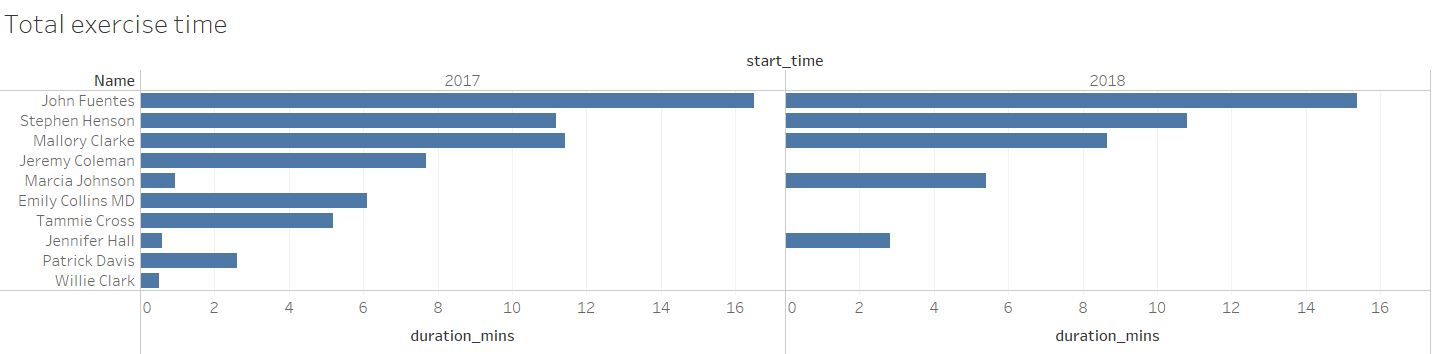
\includegraphics[width=1\linewidth]{gfx/Total_exercise_time}
	\caption{Class exercise time year over year comparison}
	\label{fig:Total_exercise_time}
\end{figure}

If the interest is on when do the students practice, a visualization by weekday can show us that, for example, for a particular class, most of the students prefer to practice on Wednesday (Figure \ref{fig:Class_exercise_by_weekday}).

\begin{figure}[bth]
	\centering
	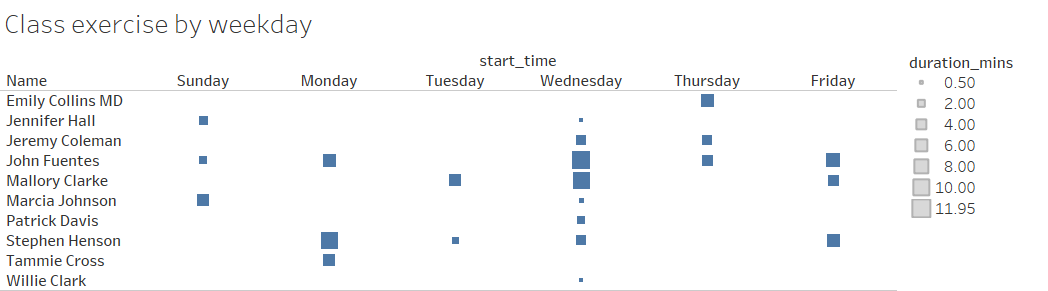
\includegraphics[width=1\linewidth]{gfx/Class_exercise_by_weekday}
	\caption{Class exercise heatmap by weekday}
	\label{fig:Class_exercise_by_weekday}
\end{figure}

For understanding the quality of the practice, we can also visualize the average session length. An interesting finding, as we can see in Figure \ref{fig:Avg_exercise_session_duration}, is that on average the exercise sessions are 2.2 minutes long. Some of the students however practice for less than a minute, this can tell us about their commitment with the activity or about their knowledge, since exercises have fixed number of questions, and thus, a fast student will finish faster. By observing these results a teacher can encourage the class to practice for at least a certain amount of minutes in a row, in order to keep a better focus. Finally, this visualization can also be used to avoid students gaming the system by opening the application multiple times but not really focusing on the assignment.

\begin{figure}[bth]
	\centering
	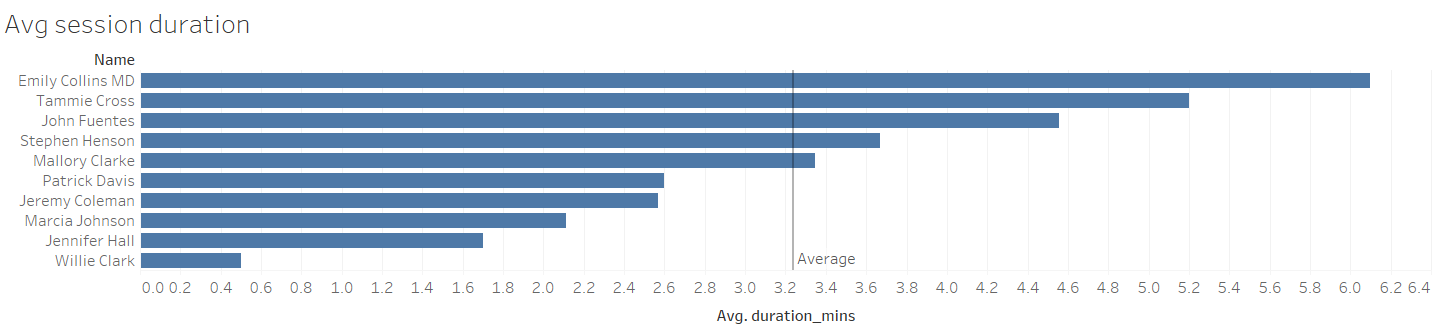
\includegraphics[width=1\linewidth]{gfx/Avg_exercise_session_duration}
	\caption{Bar chart showing average session duration by student}
	\label{fig:Avg_exercise_session_duration}
\end{figure}

Continuing with the analysis of the working habits, a detailed time line (Figure \ref{fig:Exercise_timeline}) is a more fine grained visualization, where a teacher can observe at what time of the day the students practiced and if they worked uninterruptedly or not.

\begin{figure}[!h]
	\centering
	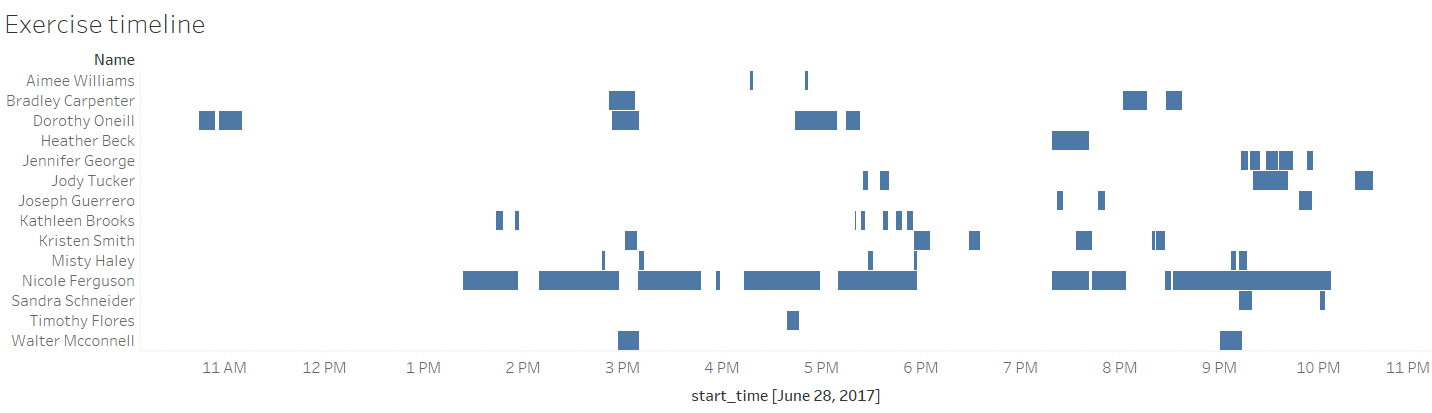
\includegraphics[width=1\linewidth]{gfx/Exercise_timeline}
	\caption{Class exercise time line}
	\label{fig:Exercise_timeline}
\end{figure}

As well, from the individual perspective, a student can observe how is his progress and consistency over time. He can set himself personal goals and track over time how is his performance. In Figure \ref{fig:Session_durations_by_user} we observe that the student was not constant in his daily practice.

\begin{figure}[!h]
	\centering
	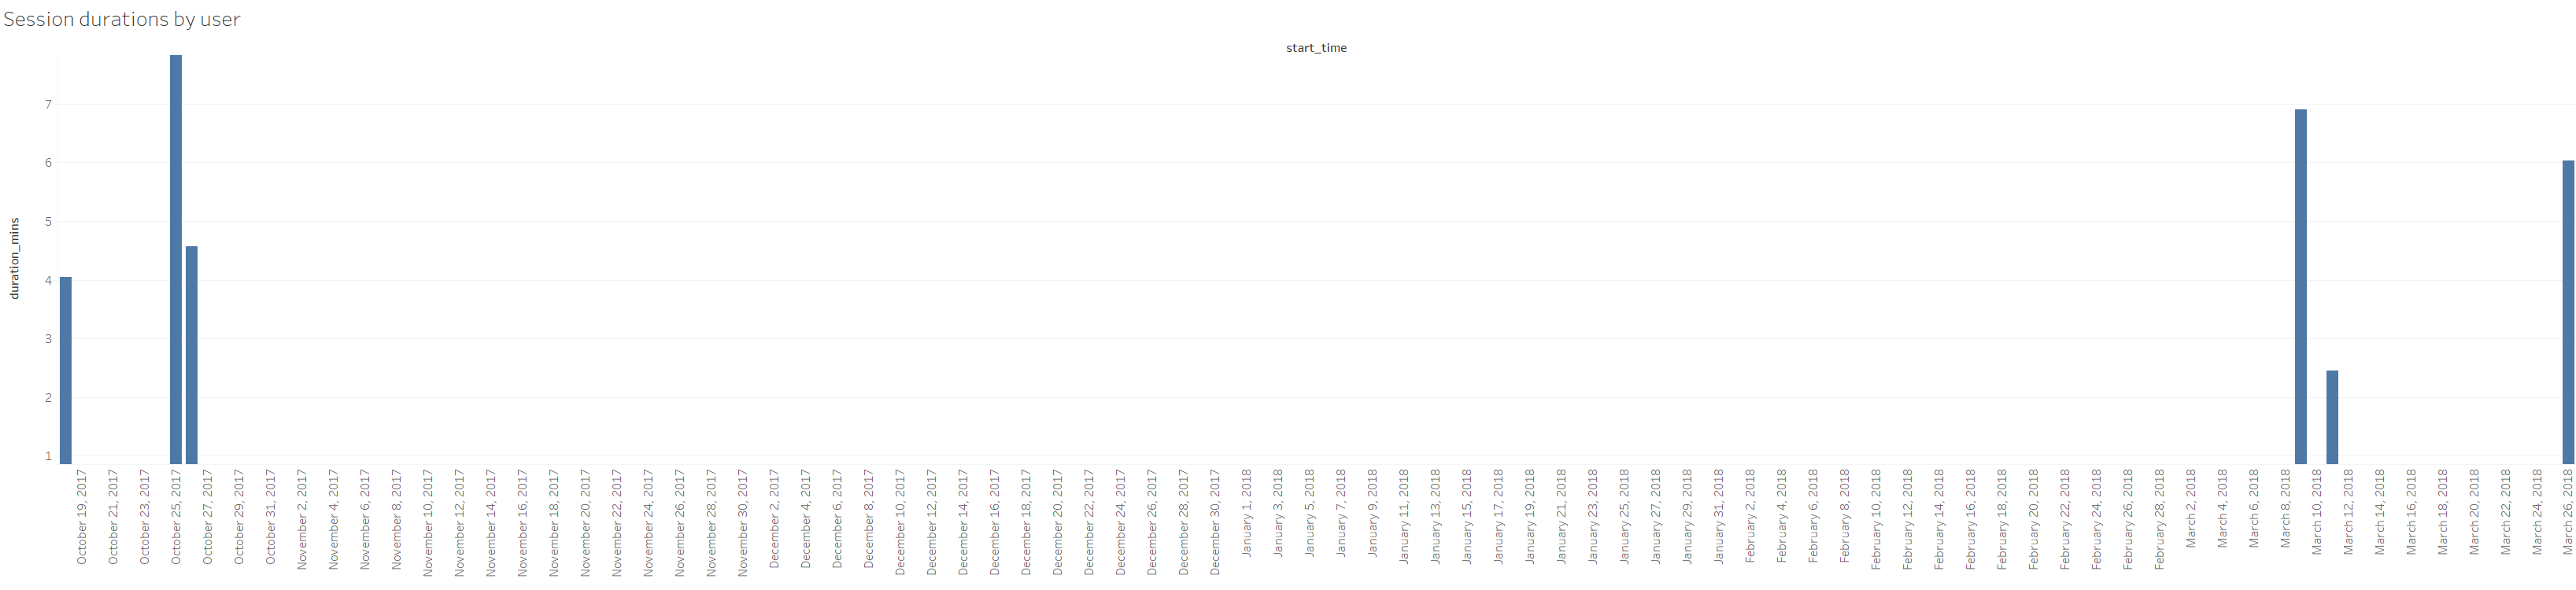
\includegraphics[width=1\linewidth]{gfx/Session_durations_by_user}
	\caption{Heat map showing exercise time calendar}
	\label{fig:Session_durations_by_user}
\end{figure}
